\documentclass[a4paper,12pt]{letter}

\usepackage{tikz}
\usepackage{amsmath}
\usepackage{amssymb}
\usepackage{nopageno}
\usepackage{amsmath}
\usepackage{enumitem}
% \usepackage{mathtools}
%\usepackage{eqnarray,amsmath}
\usepackage[a4paper, total={7.5in, 11.25in}]{geometry}
%\usepackage[margin=2.5cm]{geometry}
\usepackage[utf8]{inputenc}
\usepackage[T1]{fontenc}
\usepackage{lmodern}
%\usepackage{amsmath, amssymb}
\usepackage{setspace}
\setstretch{1.2}
\usepackage{pgfplots}
\pgfplotsset{compat=1.18}

\usetikzlibrary{calc,3d,decorations.pathmorphing,decorations.pathreplacing,decorations.markings,snakes,arrows.meta,calc,patterns}
\tikzset{snake it/.style={decorate, decoration=snake}}

\begin{document}

Name: \hrulefill\ Neptun code: \hrulefill

\bigskip

\begin{center}
(KTXFI2EBNF) Physics I. Signature Retake Exam \\
May~26,~2026
\end{center}

\bigskip
 
\begin{enumerate}[label=\Roman*.]
   
\item Mechanics

\begin{enumerate}[label=\arabic*.]
\setcounter{enumii}{0} % Számláló beállítása

% ------------------------------------------------------------------------------------------------------------------------------------

\item A projectile is launched at an angle of $60^\circ$ with an initial velocity of $100\,\text{m/s}$. 
Calculate:
\begin{enumerate}
    \item[(a)] The time to reach the peak of the trajectory.
    \item[(b)] The maximum height.
    \item[(c)] The horizontal range (impact distance).
    \item[(d)] The total time of flight.
    \end{enumerate}
($g=9.81\,\mathrm{m/s^{2}}$)     

% ------------------------------------------------------------------------------------------------------------------------------------

\item At what distance from the Uranus does an geosynchronous satellite orbit in the plane of the Equator if it remains constantly above the same point on the Uranus's surface? ($M_{Uranus}=8.68\cdot 10^{25}\,\mathrm{kg}$, $T_{Uranus}=-0,72 \,\mathrm{day}$, $R_{Uranus}=25300\,\mathrm{km}$, $G=6.6743\cdot 10^{-11}\,\mathrm{Nm^2/kg^2}$.)  

% ------------------------------------------------------------------------------------------------------------------------------------

\item A $5\,\text{kg}$ object slides down from the top of a $2\text{-meter-high}$ inclined plane that makes an angle of $15^\circ$ with the horizontal. What is the velocity of the object when it reaches the bottom of the incline, starting from rest at the top, if:
\begin{enumerate}
    \item[(a)] there is no friction between the object and the incline?
    \item[(b)] the coefficient of friction is $0.2$?
\end{enumerate}
($g=9.81\,\mathrm{m/s^{2}}$)    

% ------------------------------------------------------------------------------------------------------------------------------------

\item A string is wound around a solid cylinder with radius $R = 0.6\,\text{m}$ and mass $M = 50\,\text{kg}$. Two objects with a combined mass of $25\,\text{kg}$ are hanging from the ends of the string. Upon release, the cylinder accelerates with an angular acceleration of $\beta = 5\,\text{rad/s}^2$. The string does not slip. ($g=9.81\,\mathrm{m/s^{2}}$)     
\begin{itemize}
    \item[(a)] Find the individual masses ($m_1, m_2$) of the two objects.
    \item[(b)] Calculate the total kinetic energy of the system at $t = 5\,\text{s}$.
\end{itemize}

% ------------------------------------------------------------------------------------------------------------------------------------

\item Estimate the average depth of the Atlantic Ocean if a tsunami takes four hours to travel from Reykjavík to Lisbon. (Note: The propagation speed of shallow-water waves is $v=\sqrt{gh}$, where $g=9.81\,\mathrm{m/s^{2}}$. The distance is $3000$\,km.)

\end{enumerate}

% ------------------------------------------------------------------------------------------------------------------------------------

\item Thermodynamics

\begin{enumerate}[label=\arabic*.]
\setcounter{enumii}{5} % Számláló beállítása

% ------------------------------------------------------------------------------------------------------------------------------------

\item We place a copper piece with a mass of 500 gramms and a temperature of $40{}^{\circ}C$ into 1250 gramms of water at $70{}^{\circ}C$. What will be the common temperature? The specific heat capacity of copper is $3.85 \cdot 10^{2}\frac{J}{kg\,K}$ and the specific heat capacity of water is $4.19 \cdot 10^{3}\frac{J}{kg\,K}$.

% ------------------------------------------------------------------------------------------------------------------------------------
  
\item At a temperature of $50{}^{\circ}C$, a steel shaft with a diameter of $11.21\,cm$ needs to be fitted with an aluminum ring with an inner diameter of $11.18\,cm$ at the same temperature. The linear thermal expansion coefficient of steel is $12 \cdot 10^{-6}\frac{1}{K}$, and the linear thermal expansion coefficient of alumium is $28.7 \cdot 10^{-6}\frac{1}{K}$. What temperature should the ring be heated to?

% ------------------------------------------------------------------------------------------------------------------------------------
  
\pagebreak
\item The atmospheric balloon floating at an altitude of several kilometers has a volume of $1800\,m^{3}$. The temperature and pressure of the helium inside it are the same as the surrounding $-40{}^{\circ}C$ and $5 \cdot 10^{3}\,Pa$, respectively.
\begin{enumerate}
\item[(a)] How many moles of helium are in the balloon?
\item[(b)] What is the mass of the helium gas? $\left(M = 4 \frac{g}{mol}\right)$
\item[(c)] What was the volume of the balloon at the time of launch on Earth, if the gas inside the balloon was characterized by $0{}^{\circ}C$ and $10^{5}\,Pa$ pressure?
\end{enumerate}
($R=8.31\,\frac{J}{mol\cdot K}$)

% ------------------------------------------------------------------------------------------------------------------------------------

\item The ideal cycle of an externally heated heat engine, shown in the diagram, differs from the Otto engine cycle in that it contains isothermal processes instead of adiabatic ones.

\begin{center}
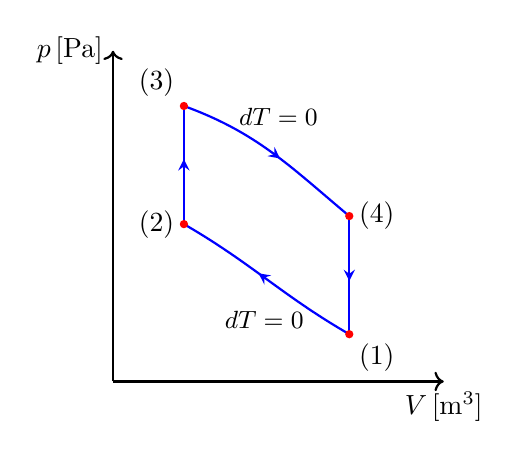
\begin{tikzpicture}[
    % Stílus a vonalak közepén elhelyezett nyilakhoz
    arrow inside/.style={
        postaction={decorate},
        decoration={
            markings,
            mark=at position 0.55 with {\arrow{stealth}}
        }
    }
,scale=0.6]

    % Tengelyek rajzolása feketével, nyilakkal a végén
    \draw[thick, ->] (0,0) -- (7,0) node[below] {$V \, [\mathrm{m^3}]$};
    \draw[thick, ->] (0,0) -- (0,7) node[left] {$p \, [\mathrm{Pa}]$};

    % Pontok koordinátáinak meghatározása
    % Úgy állítjuk be, hogy p3-p2 = p4-p1 legyen (ugyanakkora függőleges szakaszok)
    
    \coordinate (P1) at (5, 1);     % (1) Jobb alsó
    \coordinate (P2) at (1.5, 3.33); % (2) Balra fent (izoterma 1: p*V=5)
    \coordinate (P3) at (1.5, 5.83); % (3) Izochor (p3 = p2 + 2.5)
    \coordinate (P4) at (5, 3.5);    % (4) Izochor (p4 = p1 + 2.5), így p4-p1 = 2.5
    % Megjegyzés: A (3)-(4) görbe így egy másik izoterma (p*V = 1.5*5.83 = 8.75 és 5*3.5 = 17.5)
    % A fizikai hűség kedvéért a (3)-(4) ív is izotermikus marad a rajzon.

    % Folyamatok rajzolása kékkel, középen nyíllal
    % (1) -> (2): Izoterma (dT=0)
    \draw[blue, thick, arrow inside] (P1) to[out=150, in=330] (P2);
    
    % (2) -> (3): Izochor (függőleges, bal oldali)
    \draw[blue, thick, arrow inside] (P2) -- (P3);
    
    % (3) -> (4): Izoterma (dT=0)
    \draw[blue, thick, arrow inside] (P3) to[out=340, in=140] (P4);
    
    % (4) -> (1): Izochor (függőleges, jobb oldali, zárja a kört)
    \draw[blue, thick, arrow inside] (P4) -- (P1);

    % Piros pontok és címkék
    \fill[red] (P1) circle (2.5pt) node[below right, black] {(1)};
    \fill[red] (P2) circle (2.5pt) node[left, black] {(2)};
    \fill[red] (P3) circle (2.5pt) node[above left, black] {(3)};
    \fill[red] (P4) circle (2.5pt) node[right, black] {(4)};

    % Feliratok: dT=0 feketével az izotermák mellett
    \node[black, font=\small] at (3.2, 1.3) {$dT=0$}; 
    \node[black, font=\small] at (3.5, 5.6) {$dT=0$};
\end{tikzpicture}
\end{center}
What is the efficiency of the cycle if $p_{3} = 2 p_{2}$ , the compression ratio is 8, and the cycle is performed with a two-atomic (diatomic) gas? What is the efficiency of the Carnot cycle taking place between the same temperature limits? ($R=8.31\,\frac{J}{mol\cdot K}$)

% ------------------------------------------------------------------------------------------------------------------------------------

\item What is the entropy change if the volume of $ m = 2\,\mathrm{g} $ of hydrogen changes from $ V_1 = 30\,\mathrm{l} \text{\ to\ } V_2 = 120\,\mathrm{l},$ and its temperature changes from $t_1 = 80^\circ\mathrm{C} \text{\ to\ } t_2 = 400^\circ\mathrm{C}$? The molar mass is $ M = 2\,\mathrm{g/mol}$, $R=8.31\,\frac{J}{mol\cdot K}$.
  
\end{enumerate}
  
% ------------------------------------------------------------------------------------------------------------------------------------

\item Electrostatics, Waves, and Optics

\begin{enumerate}[label=\arabic*.]
\setcounter{enumii}{10} % Számláló beállítása

\item Determine the acceleration of a proton $ m = 1.67 \cdot 10^{-27}\,\mathrm{kg} $ in an electric field of strength $ E = 300\,\mathrm{N/C}. $ How many times greater is this acceleration than the acceleration due to gravity? ($e=1.6\cdot 10^{-19}\,C$, $g=9.81\,\mathrm{m/s^{2}}$) 

% ------------------------------------------------------------------------------------------------------------------------------------

\item An electron is launched with an initial velocity of $ v_0 = 3\cdot 10^6\,\mathrm{m/s} $ between two parallel charged plates, as shown in the figure. If the electric field strength between the plates is $ E = 3\,\mathrm{kN/C}, $ where does the electron hit the upper plate? Assume that the arrangement is in vacuum.

\begin{center}
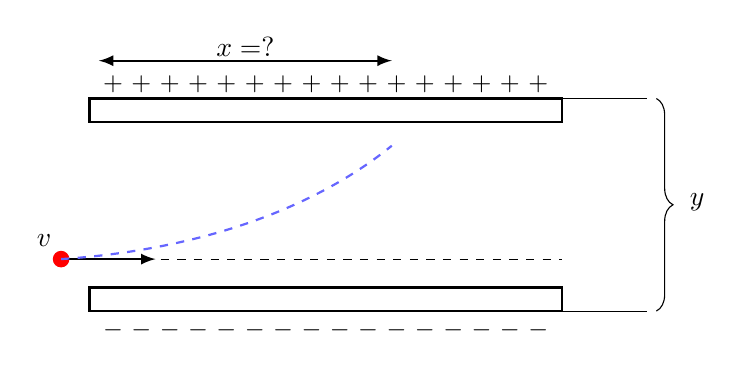
\begin{tikzpicture}[scale=1.2, >=latex]

% Plates
\draw[thick] (0,0) rectangle (5,0.25);
\draw[thick] (0,-2.0) rectangle (5,-1.75);

% Positive charges above upper plate
\foreach \x in {0.25,0.55,...,5.0}
{
    \node at (\x,0.4) {\small $+$};
}

% Negative charges below lower plate
\foreach \x in {0.25,0.55,...,5.0}
{
    \node at (\x,-2.2) {\small $-$};
}

% Electron
\fill[red] (-0.3,-1.45) circle (2.5pt);

% Initial velocity
\draw[->, thick] (-0.25,-1.45) -- (0.7,-1.45);
\node[left] at (-0.3,-1.25) {$v$};

% Dashed horizontal reference line
\draw[dashed] (-0.3,-1.45) -- (5.0,-1.45);

% Curved trajectory
\draw[dashed, thick, blue!60]
    (-0.3,-1.45) .. controls (1.2,-1.35) and (2.4,-0.9) .. (3.2,-0.25);

% x distance arrow
\draw[<->, thick] (0.1,0.65) -- (3.2,0.65);
\node at (1.65,0.8) {$x=?$};

% Vertical bracket for y
\draw[,thin] (5.6,0.25) -- (5.9,0.25);
\draw[thin] (5.6,-2.0) -- (5.9,-2.0);
\draw[decorate, decoration={brace, amplitude=6pt,mirror}]
    (6.0,-2.0) -- (6.0,0.25);
\node[right] at (6.25,-0.85) {$y$};

% Outer light guide lines
\draw[thin] (5.0,0.25) -- (5.6,0.25);
\draw[thin] (5.0,-2.0) -- (5.6,-2.0);

\end{tikzpicture}
%\caption{Electron motion between two parallel charged plates.}
\end{center}
($m_{e}=9.1\cdot 10^{-31}\,\mathrm{kg}$, $e=1.6\cdot 10^{-19}\,C$)

% ----------------------------------------------------------------------------------------------------------------------------------------

\pagebreak
\item An electron enters the region between the plate pair shown in the figure halfway between the plates. The length of the plates is $ l = 20\,\mathrm{cm}, $ their separation is $ d = 2\,\mathrm{cm}, $ and the voltage between them is $ U = 500\,\mathrm{V}. $ What must the initial velocity of the electron be if we want it to just barely leave the region between the plates? ($m_{e}=9.1\cdot 10^{-31}\,\mathrm{kg}$, $e=1.6\cdot 10^{-19}\,C$) 

\begin{center}
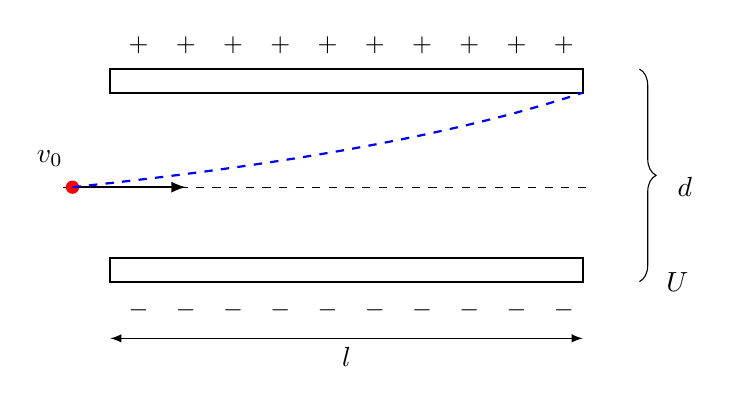
\begin{tikzpicture}[scale=1.2, >=latex]

% Parameters (for clarity)
\def\L{5}    % plate length
\def\d{2}    % plate distance

% Plates
\draw[thick] (0,0) rectangle (\L,0.25);
\draw[thick] (0,-\d) rectangle (\L,-\d+0.25);

% Positive charges (upper plate)
\foreach \x in {0.3,0.8,...,4.8}
{
    \node at (\x,+0.5) {\small $+$};
}

% Negative charges (lower plate)
\foreach \x in {0.3,0.8,...,4.8}
{
    \node at (\x,-2.3) {\small $-$};
}

% Midline (entry level)
\draw[dashed] (-0.5,-\d/2) -- (\L+0.1,-\d/2);

% Electron entry point
\fill[red] (-0.4,-\d/2) circle (2pt);

% Initial velocity
\draw[->, thick] (-0.4,-\d/2) -- (0.8,-\d/2);
\node[left] at (-0.4,-\d/2+0.3) {$v_0$};

% Curved trajectory (just touching upper plate at exit)
\draw[thick, dashed, blue]
    (-0.4,-\d/2) .. controls (1.5,-\d/2+0.2) and (3.5,-0.5) .. (\L,0.0);

% Length l
\draw[<->] (0,-\d-0.6) -- (\L,-\d-0.6);
\node at (\L/2,-\d-0.8) {$l$};

% Distance d (brace)
\draw[decorate, decoration={brace, amplitude=6pt, mirror}]
    (\L+0.6,-\d) -- (\L+0.6,0.25);
\node[right] at (\L+0.9,-\d/2) {$d$};

% Voltage label
\node at (\L+1.0,-\d/2-1.0) {$U$};

\end{tikzpicture}
%\caption{Electron motion between parallel plates (Problem 3).}
\end{center}

\end{enumerate}

\end{enumerate}

% ------------------------------------------------------------------------------------------------------------------------------------

Grades: Rejected, Teacher's signature. 

\rightline{Dr.~Gabor FACSKO}
\rightline{\textit{facsko.gabor@uni-obuda.hu}}

\vfill

\end{document}
